\documentclass[12pt, a4paper, twoside]{article}
\usepackage[utf8]{inputenc}
\usepackage[cm]{fullpage}
\usepackage{fancyhdr}
\usepackage{textcomp}
\usepackage{graphicx}

\begin{document}

\title{Relatório do Experimento 3 de OAC}
\author{
Arthur Bizzi: 13/0102636 \\
Arthur da Silveira Couto: 16/0002575 \\
Caio Albuquerque Brandão: 16/0003636 \\
Cristiano Silva Júnior: 13/0070629 \\
Leonardo Maffei: 16/0033811 \\}
\date{7 de Junho de 2017}
\maketitle

\section{Exercício 1}

\subsection{Parte A}

\subsection{Exercício 4}

O código no arquivo \textit{SYSTEMv53.s} descreve uma rotina de tratamento de exceções, como evidenciado na figura 1.

% Como adicionar uma figura
\begin{figure}
    \centering
    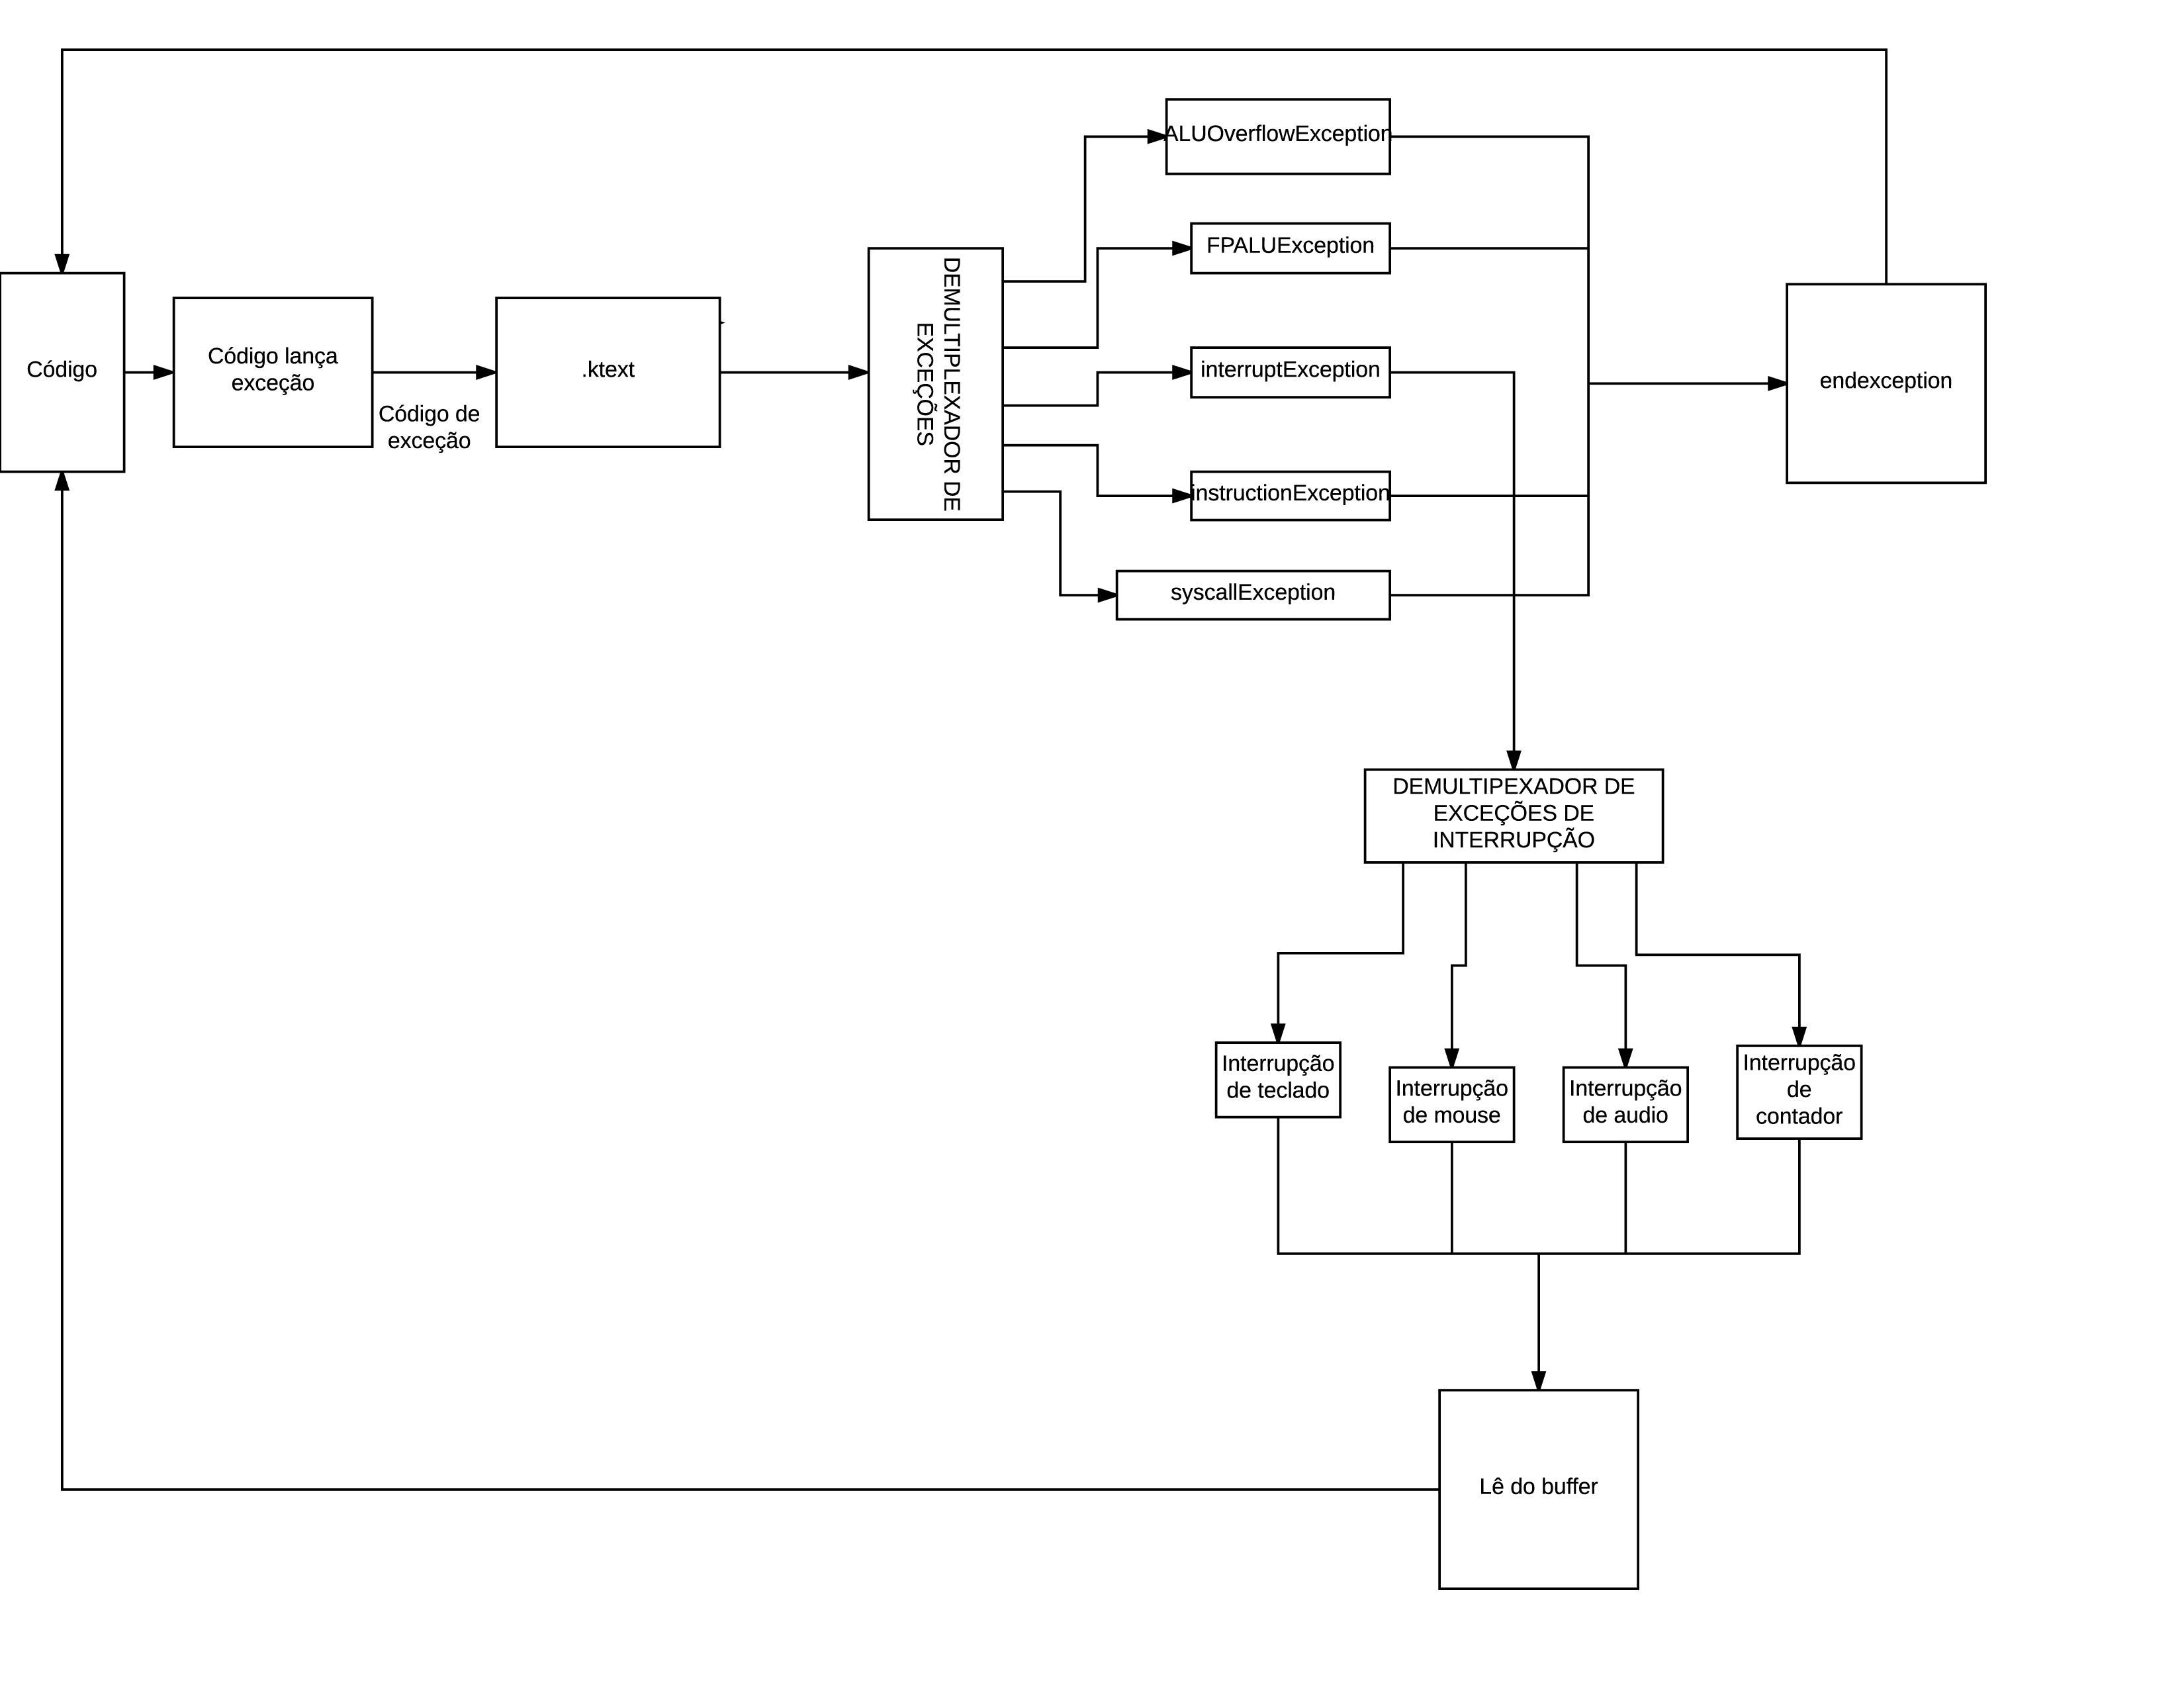
\includegraphics[width=0.8\textwidth]{./figs/f1-4.png}
    \caption{Diagrama do fluxo de tratamento de exceções}
\end{figure}

\section{Parte B}

% TODO Fazer questão 2 do relatório
\subsection{Exercício 7}

Analisando o código em \textit{Verilog} do processador descrito no projeto \textit{MIPS-PUM-v4.8}, podemos construir o diagrama de blocos presente na figura 2 para descrever a estrutura do processador a nível de estruturas funcionais.

\begin{figure}
    \centering
    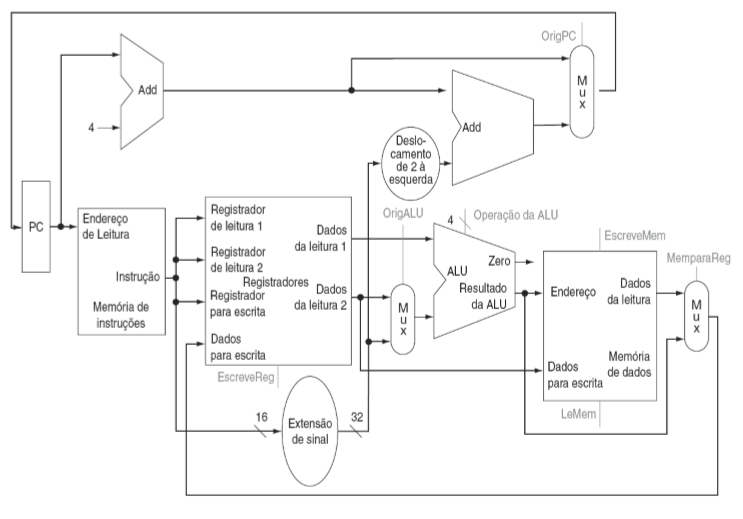
\includegraphics[width=0.8\textwidth]{./figs/q7.png}
    \caption{Diagrama de blocos do processador uniciclo}
\end{figure}

% TODO Gerar uma figura própria.

\subsection{Exercício 8}

Criar um programa \textit{teste.s} para testar todos os comandos do processador.

\subsection{Exercício 9}

Checar o tamanho do processador com e sem a FPULA.

\subsection{Exercício 10}

Implementar as funções \textit{ceil}, \textit{floor} e \textit{round}.





\end{document}
